\documentclass{beamer}
\usetheme{Boadilla}

\makeatother
\setbeamertemplate{footline}
{
    \leavevmode%
    \hbox{%
    \begin{beamercolorbox}[wd=.4\paperwidth,ht=2.25ex,dp=1ex,center]{author in head/foot}%
        \usebeamerfont{author in head/foot}\insertshortauthor
    \end{beamercolorbox}%
    \begin{beamercolorbox}[wd=.55\paperwidth,ht=2.25ex,dp=1ex,center]{title in head/foot}%
        \usebeamerfont{title in head/foot}\insertshorttitle
    \end{beamercolorbox}%
    \begin{beamercolorbox}[wd=.05\paperwidth,ht=2.25ex,dp=1ex,center]{date in head/foot}%
        \insertframenumber{}
    \end{beamercolorbox}}%
    \vskip0pt%
}
\makeatletter
\setbeamertemplate{navigation symbols}{}

\usepackage{lmodern}
\usepackage{amssymb,amsmath}
\renewcommand{\familydefault}{\sfdefault}

\DeclareMathOperator*{\argmax}{argmax}

\usepackage{mathtools}
\usepackage{graphicx}
\usepackage{threeparttable}
\usepackage{booktabs}
\usepackage{siunitx}
\sisetup{parse-numbers=false}

% \setlength{\OuterFrameSep}{-2pt}
% \makeatletter
% \preto{\@verbatim}{\topsep=-10pt \partopsep=-10pt }
% \makeatother

\title[Week 1:\ Structural Estimation]{Week 1:\ Structural Estimation}
\author[ResEcon 703:\ Advanced Econometrics]{ResEcon 703:\ Topics in Advanced Econometrics}
\date{Matt Woerman\\University of Massachusetts Amherst}

\begin{document}

{\setbeamertemplate{footline}{} 
\begin{frame}[noframenumbering]
    \titlepage
\end{frame}
}

\section{Agenda}
\begin{frame}\frametitle{Agenda}
    This week's topics
    \begin{itemize}
    	\item \hyperlink{page.\getpagerefnumber{overview}}{Course overview}
        \item \hyperlink{page.\getpagerefnumber{what}}{What is structural econometrics?}
        \item \hyperlink{page.\getpagerefnumber{why}}{Why add structure to an econometric model?}
        \item \hyperlink{page.\getpagerefnumber{how}}{How to construct a structural econometric model}
        \item \hyperlink{page.\getpagerefnumber{mw}}{Miller and Weinberg (2017)}
    \end{itemize}
    \vspace{2ex}
    This week's reading
    \begin{itemize}
        \item Nevo and Whinston (2010)
    \end{itemize}
\end{frame}

\section{Course Overview}
\label{overview}
\begin{frame}\frametitle{}
    \vfill
    \centering
    \begin{beamercolorbox}[center]{title}
        \Large Course Overview
    \end{beamercolorbox}
    \vfill
\end{frame}

\begin{frame}\frametitle{Course Goals}
    \begin{enumerate}
        \item Gain an in-depth understanding of some of the most common structural estimation methods in modern empirical economics
        \begin{itemize}
            \item Maximum likelihood estimation
            \item Generalized method of moments
            \item Maximum simulated likelihood
            \item Method of simulated moments
        \end{itemize}
        \vspace{2ex} 
        \item Develop the technical ability to apply these structural estimation methods to your own research
        \vspace{2ex}
        \item Apply these methods to discrete choice models motivated by the random utility model
        \begin{itemize}
            \item Logit model
            \item Generalized extreme value models (nested logit model)
            \item Mixed logit model (random coefficients logit model)
        \end{itemize}
    \end{enumerate}
\end{frame}

\begin{frame}\frametitle{Course Website}
    \begin{center}
        \href{https://github.com/woerman/ResEcon703}{\texttt{github.com/woerman/ResEcon703}}
    \end{center}
    \vspace{3ex}
    I will use this GitHub repository to post lecture slides, R code, links to lecture videos, problem sets, datasets, etc.
\end{frame}

\begin{frame}\frametitle{Textbook}
    \begin{tabular}{cl}  
        \begin{tabular}{c}
            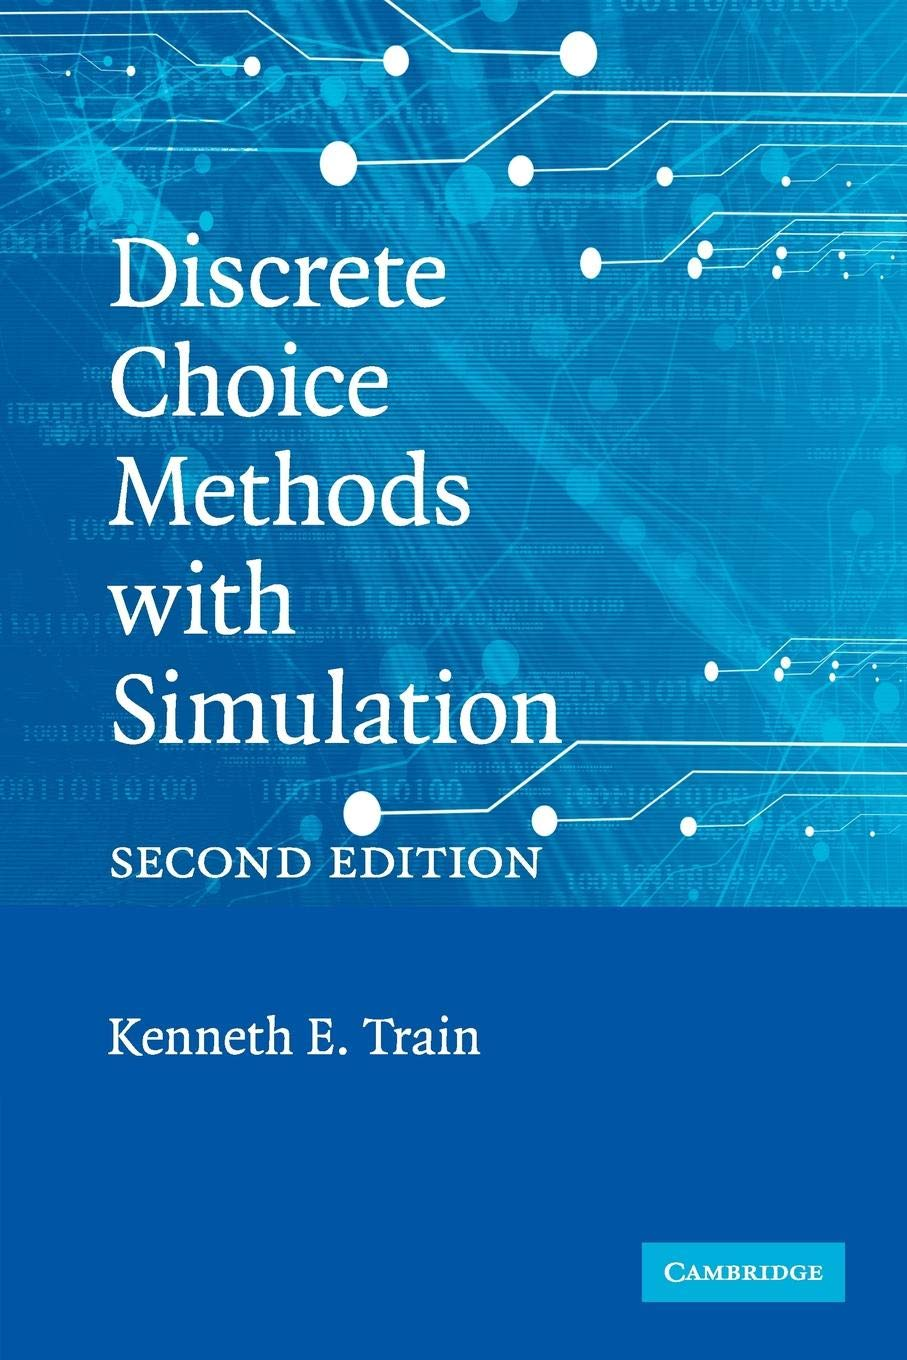
\includegraphics[width=0.2\linewidth]{train}
        \end{tabular} & 
        \begin{tabular}{l}
            \parbox{0.65\linewidth}{
            \emph{Discrete Choice Methods with Simulation\\ (Second Edition)}\\ Kenneth E.\ Train
            \begin{itemize}
                \item Available for free at: \href{https://eml.berkeley.edu/books/choice2.html}{\texttt{eml.berkeley.edu/books/choice2.html}}
                \item Paperback copy is usually less than $\$50$
            \end{itemize}
            }
        \end{tabular}
    \end{tabular} \\
    \vspace{3ex}
    \begin{itemize}
    	\item I will also post supplemental notes on some topics that we cover
    \end{itemize}
\end{frame}

\begin{frame}\frametitle{Other References}
    \begin{tabular}{cl}  
        \begin{tabular}{c}
            
\includegraphics[width=0.1\linewidth]{cameron}
        \end{tabular} & 
        \begin{tabular}{l}
            \parbox{0.75\linewidth}{
            \emph{Microeconometrics:\ Methods and Applications}\\ A. Colin Cameron and Pravin K. Trivedi
            }
        \end{tabular}
    \end{tabular} \\
    \vspace{1ex}
    \begin{tabular}{cl}  
        \begin{tabular}{c}
            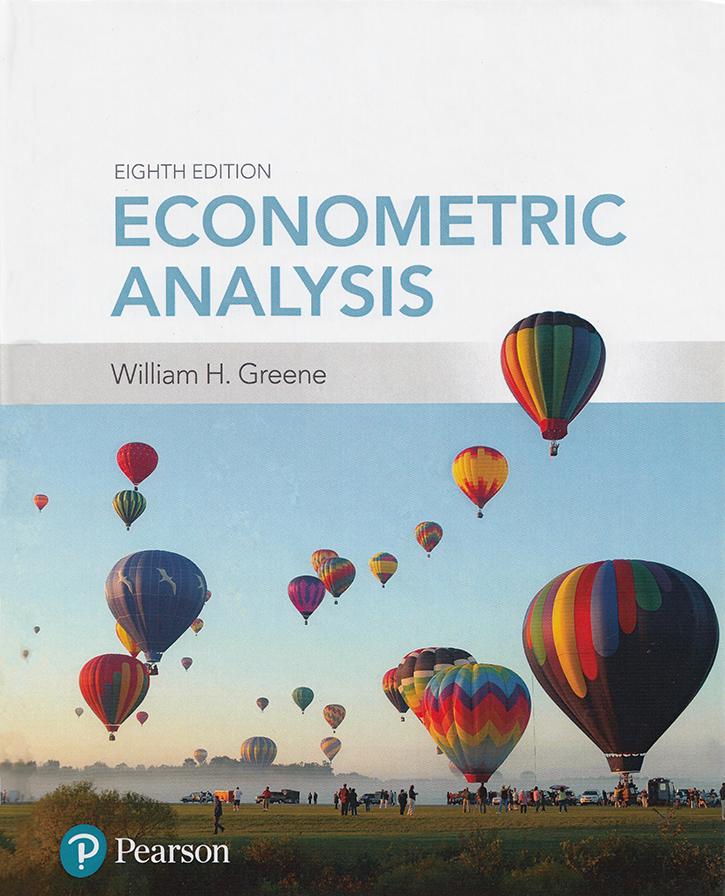
\includegraphics[width=0.1\linewidth]{greene}
        \end{tabular} & 
        \begin{tabular}{l}
            \parbox{0.75\linewidth}{
            \emph{Econometric Analysis}\\ William H. Greene
            }
        \end{tabular}
    \end{tabular} \\
    \vspace{1ex}
    \begin{tabular}{cl}  
        \begin{tabular}{c}
            
\includegraphics[width=0.1\linewidth]{hayashi}
        \end{tabular} & 
        \begin{tabular}{l}
            \parbox{0.75\linewidth}{
            \emph{Econometrics}\\ Fumio Hayashi
            }
        \end{tabular}
    \end{tabular} \\
    \vspace{1ex}
    \begin{tabular}{cl}  
        \begin{tabular}{c}
            
\includegraphics[width=0.1\linewidth]{wooldridge}
        \end{tabular} & 
        \begin{tabular}{l}
            \parbox{0.75\linewidth}{
            \emph{Econometric Analysis of Cross Section and Panel Data}\\ Jeffrey M. Wooldridge
            }
        \end{tabular}
    \end{tabular}
\end{frame}

\begin{frame}\frametitle{Software}
    We will use the R statistical programming language in this course \\
    \vspace{2ex}
    But I already know Stata/Matlab/Python/SAS/Julia. Why R?
    \begin{itemize}
        \item R is free and open source
        \item R is powerful and flexible
        \begin{itemize}
            \item Basic statistics, data cleaning, linear regression, matrix algebra, simulation methods, structural estimation, data visualization, etc.
        \end{itemize}
        \item R is favored by employers
    \end{itemize}
    \vspace{2ex}
    How can I learn R?
    \begin{itemize}
        \item R tutorial next week
        \item Many R resources available for free
        \item First problem set will be a (relatively) gentle introduction to R
    \end{itemize}
\end{frame}

\begin{frame}\frametitle{Installing R}
    Installing R is \emph{usually} straightforward \\
    \vspace{1ex}
    \begin{tabular}{@{\extracolsep{-2ex}} c l}
        \begin{tabular}{c}
            
\includegraphics[width=0.05\linewidth]{r}
        \end{tabular} & 
        \begin{tabular}{l}
            \parbox{0.9\linewidth}{
            \href{https://cran.r-project.org/}{Download (\texttt{cran.r-project.org})} and install R
            }
        \end{tabular}
    \end{tabular} \\
    \vspace{1ex}
    \begin{tabular}{@{\extracolsep{-2ex}} c l}
        \begin{tabular}{c}
            
\includegraphics[width=0.05\linewidth]{rstudio}
        \end{tabular} & 
        \begin{tabular}{l}
            \parbox{0.9\linewidth}{
            \href{https://www.rstudio.com/products/rstudio/download/}{Download (\texttt{www.rstudio.com/products/rstudio/download})}\\ and install RStudio Desktop (Open Source License)
            }
        \end{tabular}
    \end{tabular} \\
    \vspace{3ex}
    What is the difference between R and RStudio? \\
    \vspace{1ex}
    \begin{tabular}{@{\extracolsep{-2ex}} c l}
        \begin{tabular}{c}
            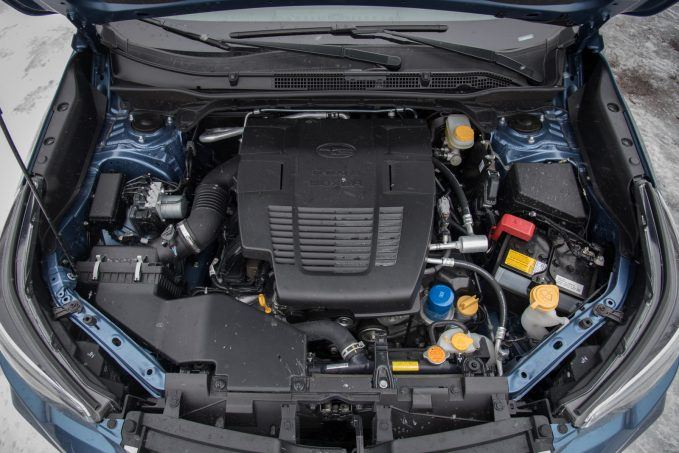
\includegraphics[width=0.25\linewidth]{engine}
        \end{tabular} & 
        \begin{tabular}{l}
            \parbox{0.65\linewidth}{
            R is like a car's engine. It is the program that powers your data analysis.
            }
        \end{tabular}
    \end{tabular} \\
    \vspace{1ex}
    \begin{tabular}{@{\extracolsep{-2ex}} c l}
        \begin{tabular}{c}
            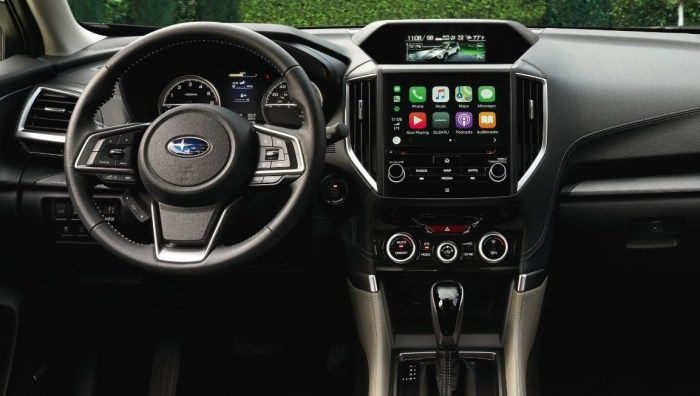
\includegraphics[width=0.25\linewidth]{dashboard}
        \end{tabular} & 
        \begin{tabular}{l}
            \parbox{0.65\linewidth}{
            RStudio is like a car's dashboard. It is the program you interact with to harness the power of your ``engine.''
            }
        \end{tabular}
    \end{tabular}
\end{frame}

\section{What Is Structural Econometrics?}
\label{what}
\begin{frame}\frametitle{}
    \vfill
    \centering
    \begin{beamercolorbox}[center]{title}
        \Large What Is Structural Econometrics?
    \end{beamercolorbox}
    \vfill
\end{frame}

\begin{frame}\frametitle{What is Structural Econometrics?}
    Many definitions! \\
    \vspace{3ex}
    Heckman and Vytlacil (2007)
    \begin{itemize}
    	\item Summarize four definitions of ``structure'' in econometrics that have been used over the last 70+ years
    \end{itemize}
    \vspace{3ex}
    Reiss and Wolak (2007)
    \begin{itemize}
    	\item ``Today economists refer to models that combine explicit economic theories with statistical models as \emph{structural econometric models}.''
    \end{itemize}
    \vspace{3ex}
    Nevo and Whinston (2010)
    \begin{itemize}
    	\item ``Structural modeling attempts to use data to identify the parameters of an underlying economic model, based on models of individual choice or aggregate relations derived from them.''
    \end{itemize}
\end{frame}

\begin{frame}\frametitle{Structural Econometric Model}
    Economic theory
    \begin{itemize}
        \item Tells us how a set of observed endogenous variables ($y$) are related to a set of observed exogenous variables ($x$)
        \item May also relate the endogenous variables to unobserved variables ($\xi$)
        \item Specifies a functional form ($g()$) and unknown parameters ($\Theta$)
    \end{itemize}
    \vspace{1ex}
    $$y = g(x, \xi, \Theta)$$ \\
    \vspace{2ex}
    Statistical assumptions
    \begin{itemize}
        \item Give a joint distribution of $x$ and $\xi$
    \end{itemize}
    \vspace{1ex}
    $$f(x, \xi)$$ \\
    \vspace{2ex}
    Estimating equation
    \begin{itemize}
    	\item Log-likelihood function, conditional moments, etc.
    \end{itemize}
    \vspace{1ex}
    $$\ell(y, x \mid \Theta) \quad \text{or} \quad E(y \mid x, \Theta)$$
\end{frame}

\begin{frame}\frametitle{Nonstructural Econometric Model}
    Nonstructural econometric models are usually grounded in economic theory but do not incorporate it so directly
    \begin{itemize}
    	\item Theory determines what variables to include in $y$ and $x$
    	\item Typically the researcher estimates the joint density of $y$ and $x$ (or something related to this joint density)
    	\item But this joint density may not have an ``economic'' interpretation
    \end{itemize}
	\vspace{2ex}
	Nonstructural econometric models may or may not be based on formal statistical models
    \begin{itemize}
    	\item Measurement studies that construct and summarize data
    	\item Autoregressive conditional heteroskedasticity (ARCH) models
    	\item Everything in-between
    \end{itemize}
    \vspace{2ex}
	There is not an absolute dichotomy of structural vs.\ nonstructural
	\begin{itemize}
		\item Not uncommon to combine structural and nonstructural approaches
	\end{itemize}
\end{frame}

\begin{frame}\frametitle{Nonstructural Auction Example}
    We observe the winning bid and the number of bidders from many auctions, and we want to understand the relationship between the number of bidders and the winning bid \\
    \vspace{2ex}
    Nonstructural (``reduced-form'') approach
    \begin{itemize}
        \item Regress winning bid on number of bidders
        \item No economic theory, microeconomic fundamentals, etc.
    \end{itemize}
    \vspace{2ex}
    Suppose you estimate a marginal effect of \$100 per bidder
    \begin{itemize}
    	\item Is this a causal estimate? No!
    	\item What use is this estimate? What can we do with it?
    \end{itemize}
    \vspace{2ex}
    Maybe you find a clever research design to estimate a causal effect
    \begin{itemize}
    	\item IV with an exogenous policy change or RD in auction rules
    	\item Does a causal estimate of \$100 per bidder tell us anything about the underlying valuations, preference, or behavior of bidders?
    \end{itemize}
\end{frame}

\begin{frame}\frametitle{Structural Auction Example}
    We observe the winning bid and the number of bidders from many auctions, and we want to understand the relationship between the number of bidders and the winning bid \\
    \vspace{2ex}
    Structural approach
    \begin{itemize}
        \item Incorporate economic and institutional details into relationship
        \item Combine auction theory with statistical assumptions to estimate underlying (and unobserved) distribution of valuations, risk preferences, etc.
    \end{itemize}
    \vspace{2ex}
    What can we do with these estimated distributions/parameters?
    \begin{itemize}
    	\item Plug these estimated distributions and parameters into the structural economic model to simulate expected auction outcomes under different numbers of bidders, different rules, etc.
    \end{itemize}
\end{frame}

\section{Why Add Structure to an Econometric Model?}
\label{why}
\begin{frame}\frametitle{}
    \vfill
    \centering
    \begin{beamercolorbox}[center]{title}
        \Large Why Add Structure to an Econometric Model?
    \end{beamercolorbox}
    \vfill
\end{frame}

\begin{frame}\frametitle{Why Add Structure to an Econometric Model?}
	Structural models can be used to:
	\begin{itemize}
		\item Estimate unobserved economic or behavioral parameters that cannot be estimated in a nonstructural (reduced-form) model
		\begin{itemize}
			\item For example: marginal utility, marginal cost, risk preferences, discount rates, search costs, switching costs, etc.
		\end{itemize}
		\item Conduct counterfactual simulations
		\begin{itemize}
			\item What would happen if the economic environment changed?
			\item Requires the underlying ``structural'' parameters that are invariant to the simulated change
		\end{itemize}
		\item Compare competing economic theories
		\begin{itemize}
			\item For example: Do firms set prices or quantities?
			\item Model must account for the implications of the economic theories in order to test them
		\end{itemize}
	\end{itemize}
\end{frame}

\begin{frame}\frametitle{Should You Always Add Structure?}
    Is a structural model always better than a nonstructural model?
    \begin{itemize}
        \item NO! The right approach depends on your research question, data, institutional details, etc.
    \end{itemize}
    \vspace{2ex}
    Negatives of structural models
    \begin{itemize}
    	\item Require existing economic theory appropriate for the empirical context
    	\item Often require (many) assumptions by the researcher to align economic theory with available data and tractable estimation
    	\begin{itemize}
    		\item If these assumptions are unrealistic, then the results are not credible
    	\end{itemize}
    	\item Assumptions may not be transparent to readers
    \end{itemize}
    \vspace{2ex}
    Advantages of nonstructural (reduced-form) models
    \begin{itemize}
        \item With a good research design, nonstructural models can provide
        \begin{itemize}
            \item Causal estimates
            \item Less reliance on researcher assumptions
            \item Transparent assumptions, estimation, and results
        \end{itemize}
        \item Without a good research design, advantages are less clear
    \end{itemize}
\end{frame}

\begin{frame}\frametitle{Structure and Credibility: Complements or Substitutes?}
    Is there always a tradeoff between structure and credibility?
    \begin{itemize}
    	\item NO! In some cases, adding structure may be the only way to credibly answer your research question
    \end{itemize}
    \vspace{2ex}
    Examples where structure adds credibility to research
    \begin{itemize}
    	\item Generalization to other settings
    	\item Out-of-sample counterfactual simulations
    	\item Welfare calculations
    \end{itemize}
    \vspace{2ex}
    Reduced-form treatment effects may not be applicable for out-of-sample extrapolation or for plugging into an economic model
    \begin{itemize}
     	\item Structural parameters are more likely to be invariant to the setting and relevant for welfare calculations
     \end{itemize} 
     \vspace{2ex}
     Merger analysis is a classic example of credibility through structure
\end{frame}

\begin{frame}\frametitle{Nonstructural Merger Analysis}
    We want to predict the welfare effects of a horizontal merger \\
    \vspace{2ex}
    Nonstructural approach
    \begin{itemize}
    	\item Estimate the effect of ``similar'' mergers on prices
    	\item Use estimated price effect in a ``back-of-the-envelope'' welfare calculation
    \end{itemize}
    \vspace{2ex}
    Potential problems with this approach
    \begin{itemize}
    	\item What counts as a ``similar'' merger? Similar industry, concentration, demand elasticity, cost structure?
    	\item Are there a sufficient number of ``similar'' mergers?
    	\item What is the control group? Or is it simply an event study of these mergers?
    	\item Are these mergers (quasi-)exogenous?
    \end{itemize}
\end{frame}

\begin{frame}\frametitle{Structural Merger Analysis}
    We want to predict the welfare effects of a horizontal merger \\
    \vspace{2ex}
    Structural approach
    \begin{itemize}
    	\item Construct an economic model of demand, supply, and competition in the industry
    	\item Estimate the structural parameters that describe the industry
    	\item Simulate the effects of the merger (including welfare effects) under a range of assumptions
    \end{itemize}
    \vspace{2ex}
    Potential problems with this approach
    \begin{itemize}
    	\item How do you credibly estimate the structural parameters? Are there valid instruments to identify every relevant parameter?
    \end{itemize}
    \vspace{2ex}
    Both approaches have strengths and limitations
\end{frame}

\begin{frame}\frametitle{Structure and Data: Complements or Substitutes?}
    If you have sufficient data to estimate credible reduced-form treatment effects, is structure still useful?
    \begin{itemize}
    	\item YES! Credible treatment effects and credible structural parameters are both useful
    \end{itemize}
    \vspace{2ex}
    Good data and identification often weaken the required assumptions
    \begin{itemize}
    	\item When the data can do more of the work, the assumptions do less heavy lifting
    	\item True for both structural and nonstructural approaches
    \end{itemize}
    \vspace{2ex}
    Combining structural and nonstructural approaches
    \begin{itemize}
    	\item Nonstructural methods can give a credible estimate of the overall treatment effect
    	\item Structural methods can help to corroborate treatment effects and identify the underlying mechanisms
    \end{itemize}
\end{frame}

\section{How to Construct a Structural Econometric Model}
\label{how}
\begin{frame}\frametitle{}
    \vfill
    \centering
    \begin{beamercolorbox}[center]{title}
        \Large How to Construct a Structural Econometric Model
    \end{beamercolorbox}
    \vfill
\end{frame}

\begin{frame}\frametitle{How to Construct a Structural Econometric Model}
    Step 1: Start with economic theory
    \begin{itemize}
        \item Description of the economic setting
        \begin{itemize}
            \item Markets, institutions, agents, information
        \end{itemize}
        \item List of primitives
        \begin{itemize}
            \item Technologies, preferences, endowments
        \end{itemize}
        \item Exogenous variables
        \begin{itemize}
            \item Constraints, regulations, shifters
        \end{itemize}
        \item Objective function and decision variables
        \begin{itemize}
            \item Utility maximization and quantities demanded, profit maximization and input quantities
        \end{itemize}
        \item Equilibrium concept
        \begin{itemize}
            \item Walrasian equilibrium with price-taking, Nash equilibrium with quantity selection
        \end{itemize}
    \end{itemize}
\end{frame}

\begin{frame}\frametitle{How to Construct a Structural Econometric Model}
    Step 2: Transform economic model into econometric model
    \begin{itemize}
        \item Unobservables that account for the data not perfectly fitting the economic model
        \begin{itemize}
            \item Researcher uncertainty about the economic setting
            \item Agent uncertainty about the economic setting
            \item Optimization error by agents
            \item Measurement error in observed variables
        \end{itemize}
    \end{itemize}
    \vspace{2ex}
    Step 3: Estimate the econometric model
    \begin{itemize}
        \item Functional forms
        \item Distribution assumptions
        \item Estimation method
        \item Specification tests
    \end{itemize}
\end{frame}

\begin{frame}\frametitle{A Simple Example of a Structural Model}
    We want to estimate the output elasticities of capital and labor for a firm
    \begin{itemize}
    	\item We observe output ($Y_t$), capital ($K_t$), and labor ($L_t$)
    \end{itemize}
    \vspace{1ex}
    \begin{enumerate}
    	\item Start with a Cobb-Douglas production function
    	$$Y_t = A K_t^\alpha L_t^\beta$$
    	Rewrite this production function as
    	$$\ln(Y_t) = \gamma + \alpha \ln(K_t) + \beta \ln(L_t)$$
    	\item Add an error term ($\varepsilon_t$) to capture measurement error and make statistical assumptions about it. (Are these assumptions reasonable?)\
        $$\varepsilon_t \sim N(0, \sigma^2) \quad \text{and} \quad E(\varepsilon_t \mid K_t, L_t) = 0$$
        \item Estimate the output elasticities $\alpha$ and $\beta$ using OLS
        $$\ln(Y_t) = \gamma + \alpha \ln(K_t) + \beta \ln(L_t) + \varepsilon_t$$
    \end{enumerate}
\end{frame}

\begin{frame}\frametitle{A More Complex Example of a Structural Model}
    We observe the winning bid ($w_t$) from $T$ procurement auctions with $N_t$ risk-neutral bidders, and we want to estimate the underlying common distribution of costs, $f(c)$, which is known to all bidders
    \begin{enumerate}
        \item Economic theory tells us each firm will maximize expected profit
        $$E[\pi_i(b_1, \ldots, b_N)] = (b_i - c_i) \Pr(b_i < b_j \; \forall j \neq i \mid c_i)$$
        Differentiate to get the first-order condition for the bid function
        $$b_i = \beta(c_i) = c_i + \frac{\int_{c_i}^\infty [1 - F(\tau)]^{N - 1} d\tau}{[1 - F(c_i)]^{N - 1}}$$
        Then the distribution of the winning bid is
        $$h(w) = \frac{N [1 - F(\beta^{-1}(w))]^{N-1} f(\beta^{-1}(w))}{\beta'(\beta^{-1}(w))}$$
    \end{enumerate}
\end{frame}

\begin{frame}\frametitle{A More Complex Example of a Structural Model}
    \begin{enumerate}\setcounter{enumi}{1}
    	\item Assume that the distribution of costs, $f(c)$, comes from a family of distributions parameterized by $\theta = (\theta_1, \theta_2, \ldots, \theta_p)$. 
    	\begin{itemize}
    		\item The lower bound of the distribution of winning bids is
    	$$\mathcal{J}(\theta, N) = \int_{0}^\infty [1 - F(\tau; \theta)]^{N - 1} d\tau$$
    	\end{itemize}\item Estimate $\theta$ using maximum likelihood subject to constraints
    	$$\hat{\theta} = \argmax_{\theta} \sum_{t = 1}^T \ln h(w_t; \theta, N_t) \text{ subject to } \mathcal{J}(\theta, N_t) \leq w_t ~ \forall t$$
    \end{enumerate}
\end{frame}

\begin{frame}\frametitle{Structural Estimation}
    Some structural models can be estimated using OLS or related regression
    \begin{itemize}
        \item Easy and fast to implement
        \item Estimation procedure and underlying assumptions are transparent
        \item Results are easily interpreted
    \end{itemize}
    \vspace{3ex}
    Some structural models require more advanced estimation methods
    \begin{itemize}
        \item Structural model cannot be simplified to a linear regression model
        \item Methods are broadly defined as ``structural estimation''
    \end{itemize}
    \vspace{3ex}
    This course will focus on ``structural estimation'' that follows from this second class of structural models
\end{frame}

\begin{frame}\frametitle{This Course}
    \begin{enumerate}
    	\item Economic model: Discrete choice to maximize utility
    	\vspace{2ex}
    	\item Econometric model: Random utility model
    	\begin{itemize}
    		\item Logit model
    		\item Generalized extreme value models (nested logit model)
    		\item Mixed logit model (random coefficients logit model)
    	\end{itemize}
    	\vspace{2ex}
    	\item Estimation methods: Structural estimation
    	\begin{itemize}
    		\item Maximum likelihood estimation
    		\item Generalized method of moments
    		\item Maximum simulated likelihood
    		\item Method of simulated moments
    	\end{itemize}
    \end{enumerate}
\end{frame}

\section{Miller and Weinberg (2017)}
\label{mw}
\begin{frame}\frametitle{}
    \vfill
    \centering
    \begin{beamercolorbox}[center]{title}
        \Large Miller and Weinberg (2017)
    \end{beamercolorbox}
    \vfill
\end{frame}

\begin{frame}\frametitle{Research Setting and Research Question}
    US beer industry
    \begin{itemize}
        \item Dominated by three larger firms: Miller, Coors, and ABI
    \end{itemize}
    \vspace{2ex}
    MillerCoors merger
    \begin{itemize}
        \item Miller and Coors combined their operations in the US through a new joint venture
        \item Merger was reviewed by US DOJ and approved in June 2008
        \begin{itemize}
            \item Some concern that increased concentration would harm consumers
            \item But cost efficiencies could reduce consumer prices
            \item DOJ determined that consumers would benefit on net
        \end{itemize}
        \item But what if the merger changed the nature of competition?
    \end{itemize}
    \vspace{2ex}
    Research question: Did the MillerCoors merger lead to new coordinated pricing between MillerCoors and ABI?
\end{frame}

\begin{frame}\frametitle{Data}
    Retail scanner data on supermarket beer sales
    \begin{itemize}
        \item Weekly revenue and unit sales by UPC code, week, and store
        \item 2001--2011, 39 geographic regions, 13 flagship brands
        \item Aggregated to region-month or region-quarter levels
    \end{itemize}
    \vspace{2ex}
    American Community Survey Public Use Microdata Sample
    \begin{itemize}
        \item Household demographics (income) for a subsample of US households
    \end{itemize}
    \vspace{2ex}
    Locations of geographic regions and breweries
    \begin{itemize}
        \item Driving distance from nearest brewery to market
    \end{itemize}
    \vspace{2ex}
    Diesel fuel prices from US EIA and US DOE
    \begin{itemize}
        \item Transportation cost to deliver goods to market
    \end{itemize}
\end{frame}

\begin{frame}\frametitle{Descriptive Evidence of Price Effects}
    \centering
    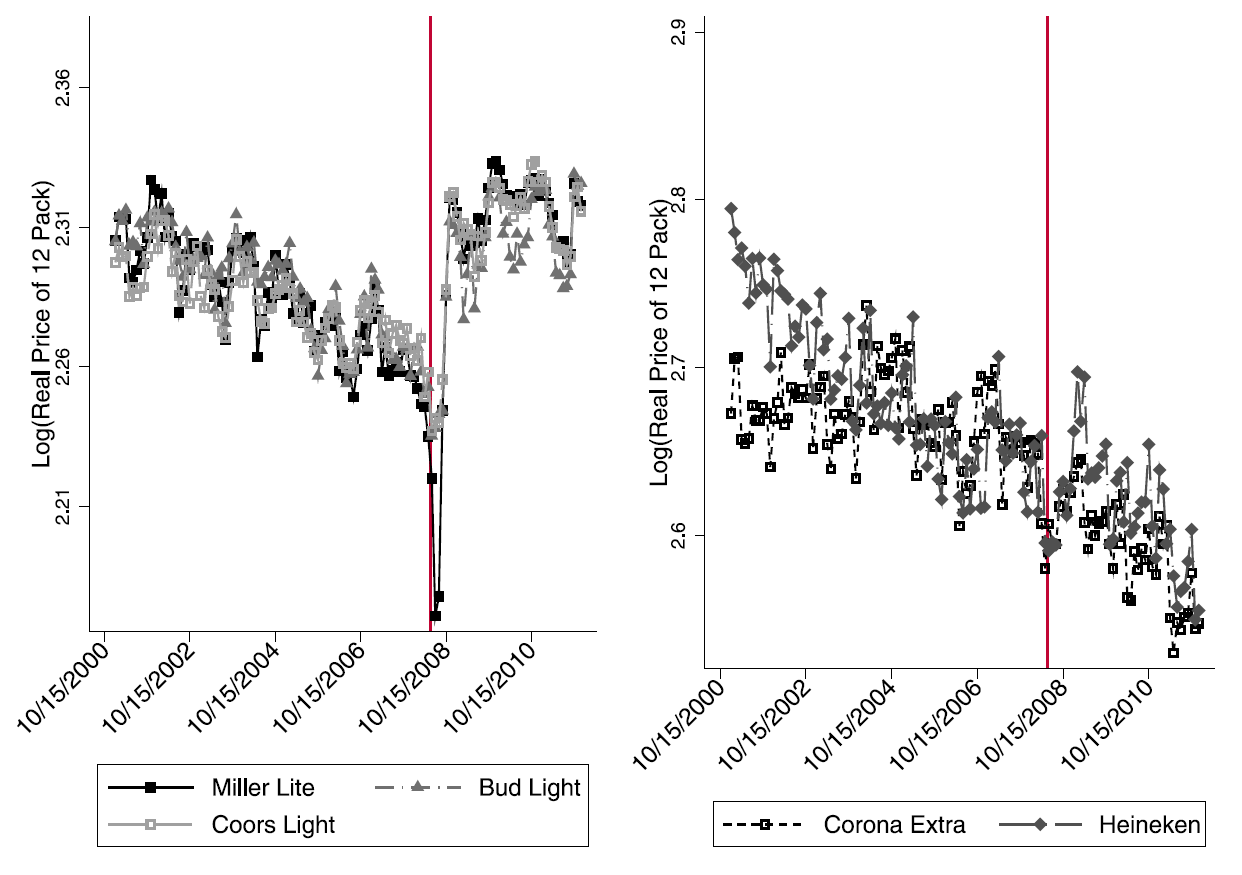
\includegraphics[width=0.95\linewidth]{fig_1}
\end{frame}

\begin{frame}\frametitle{Descriptive Evidence of Price Effects}
    After the merger, prices of Miller Lite, Coors Light, and Bud Light increase by 8\% and the downward trend ceases
    \begin{itemize}
        \item No change in price levels or trends for Corona Extra and Heineken
    \end{itemize}
    \vspace{3ex}
    This descriptive evidence is consistent with coordinated pricing by MillerCoors and ABI
    \begin{itemize}
        \item So the research question appears plausible
    \end{itemize}
    \vspace{3ex}
    But the evidence is also consistent with
    \begin{itemize}
        \item Unilateral pricing effects
        \item Institutional practices by retailers
        \item Macroeconomic conditions of the Great Recession
    \end{itemize}
\end{frame}

\begin{frame}\frametitle{Regression Evidence of Time-Series Price Effects}
    To more rigorously quantify the time-series price effects of the merger and to analyze more brands, the authors use a difference-in-differences regression design
    \vspace{2ex}
    \begin{center}
        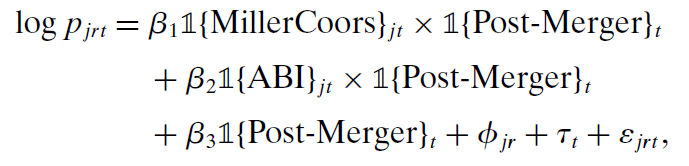
\includegraphics[width=0.5\linewidth]{eq_1}
    \end{center}
    \begin{itemize}
        \item Allow for heterogeneous effects of the merger by firm
        \item Control for cross-sectional variation and time trends
    \end{itemize}
\end{frame}

\begin{frame}\frametitle{Regression Evidence of Time-Series Price Effects}
    \begin{center}
        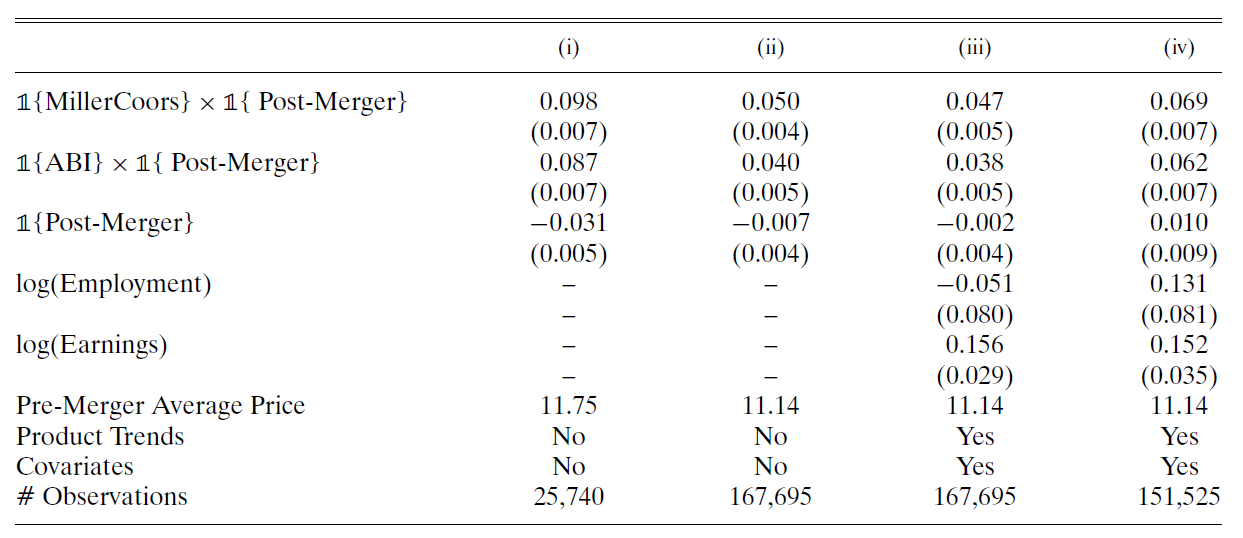
\includegraphics[width=0.95\linewidth]{table_2}
    \end{center}
    Conclusions are similar as before
    \begin{itemize}
        \item MillerCoors prices increase 5--10\% relative to import brands
        \item ABI prices increase by roughly the same amount (4--9\%)
    \end{itemize}
\end{frame}

\begin{frame}\frametitle{Regression Evidence of Cross-Sectional Price Effects}
    Under unilateral pricing, these price effects may be explained by
    \begin{itemize}
        \item Changes in industry concentration: larger price increases in markets with greater predicted increases in concentration
        \item Changes in transportation costs: smaller price increases in markets with greater transportation cost savings
    \end{itemize}
    \vspace{2ex}
    The authors use another reduced-form regression to determine how well these market-level factors explain the observed price patterns
    \vspace{2ex}
    \begin{center}
        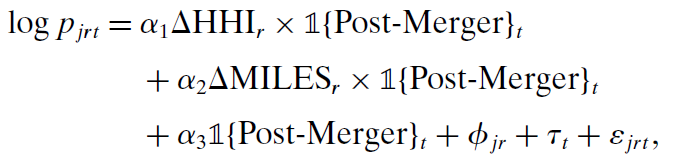
\includegraphics[width=0.5\linewidth]{eq_2}
    \end{center}
\end{frame}

\begin{frame}\frametitle{Regression Evidence of Cross-Sectional Price Effects}
    \begin{center}
        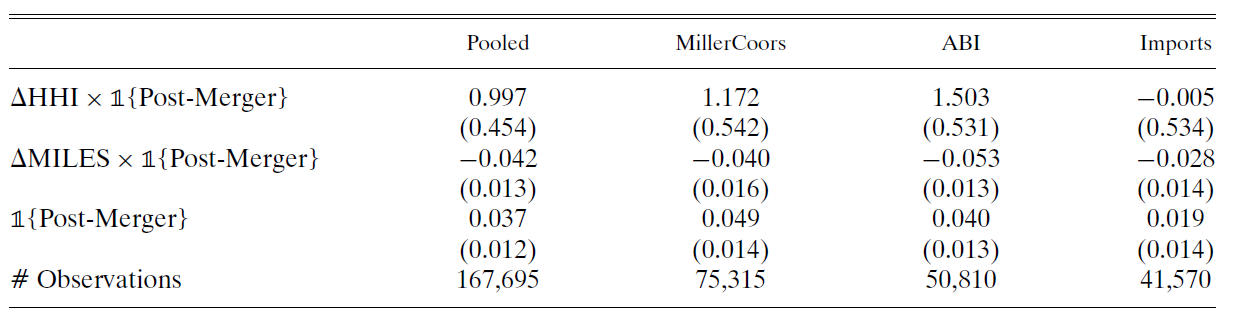
\includegraphics[width=0.95\linewidth]{table_3}
    \end{center}
    The signs of these coefficients are as expected
    \begin{itemize}
        \item MillerCoors and ABI---but not import brands---price increases are larger in markets with greater predicted increases in concentration
        \item Prices increases are smaller in markets with greater transportation cost savings
    \end{itemize}
    \vspace{2ex}
    The net effect is roughly zero on average
    \begin{itemize}
        \item Most of the price increases are not explained by these factors
        \item Unilateral effects may not explain the observed price increases
    \end{itemize}
\end{frame} 

\begin{frame}\frametitle{Additional Reduced-Form Analyses (AHW 2015)}
    Ashenfelter, Hosken, and Weinberg (2015) conduct additional reduced-from analyses of this merger to further characterize how these factors could explain unilateral price effects
    \begin{itemize}
        \item Event studies of concentration (left) and distance (right) effects
        \begin{center}
            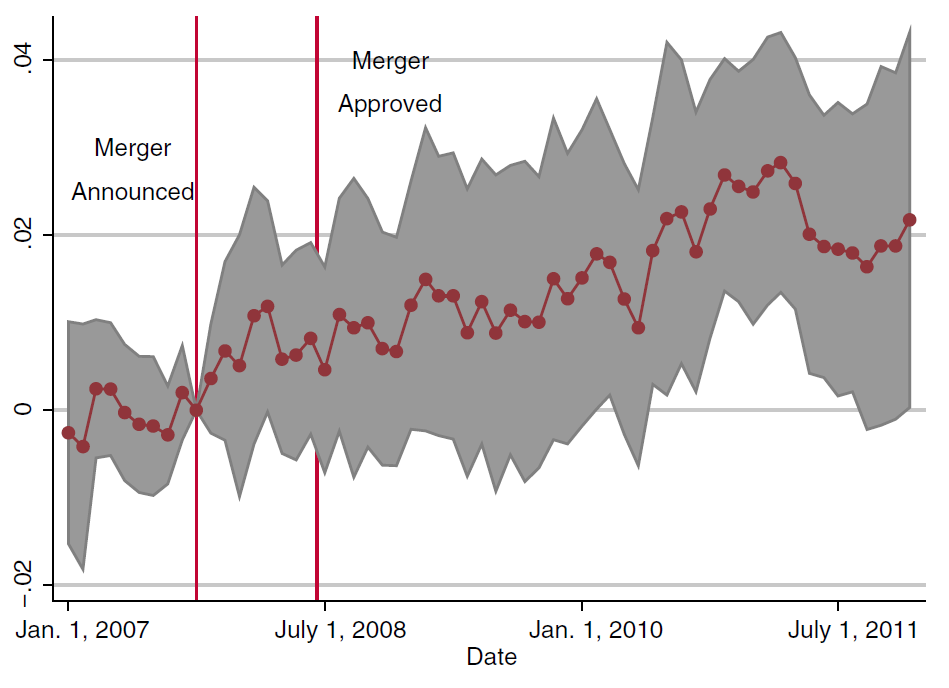
\includegraphics[width=0.25\linewidth]{ahw_fig_5}
            \hspace{8ex}
            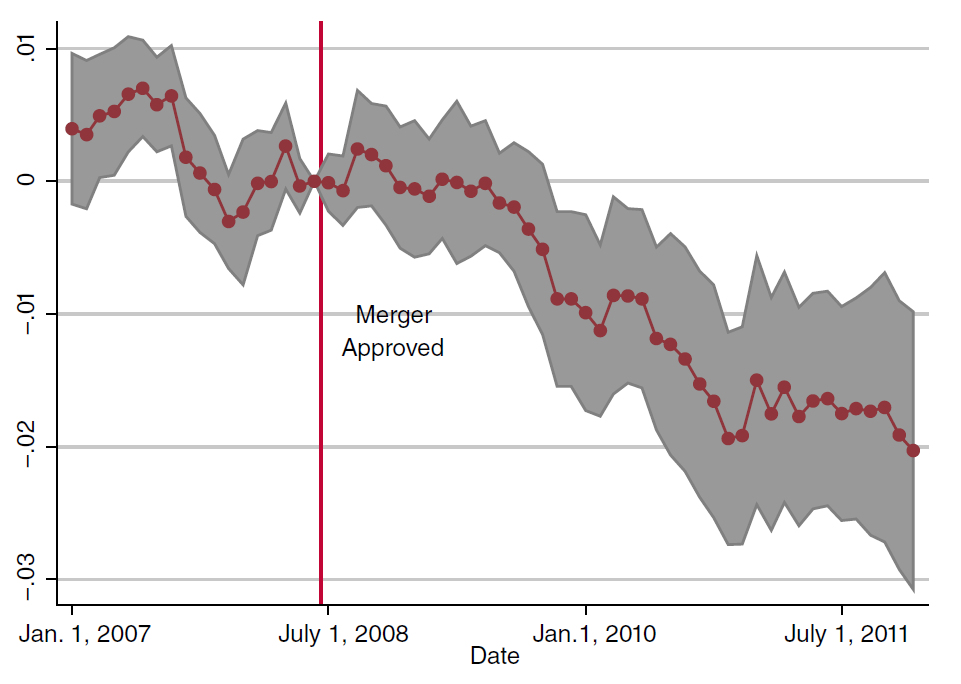
\includegraphics[width=0.25\linewidth]{ahw_fig_6}
        \end{center}
        \item Heterogeneous effects by initial market characteristics
        \begin{center}
            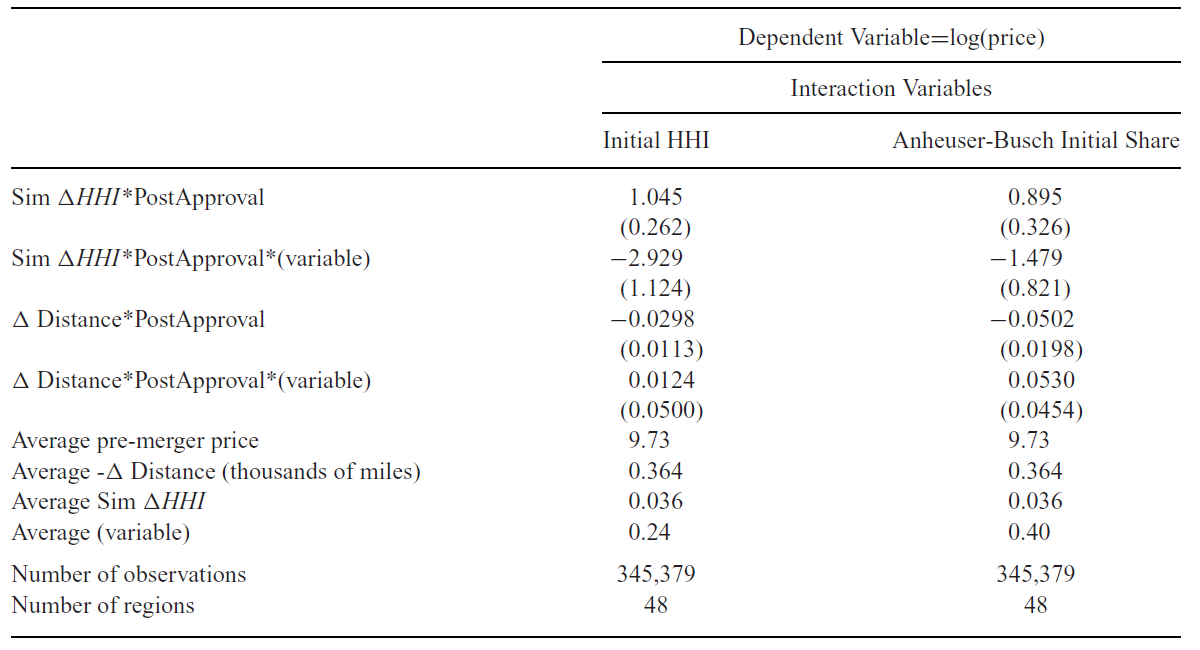
\includegraphics[width=0.5\linewidth]{ahw_table_6}
        \end{center}
    \end{itemize}
\end{frame} 

\begin{frame}\frametitle{Reduced-Form vs.\ Structural Analysis}
    Advantages of these reduced-form results
    \begin{itemize}
        \item Simple and transparent method to show substantial price effects
        \item Some evidence that prices exceed unilateral effects
    \end{itemize}
    \vspace{2ex}
    Shortcomings of these reduced-form results
    \begin{itemize}
        \item Analysis does not fully capture consumer substitution patterns, which are critical for firm pricing decisions
    \end{itemize}
    \vspace{2ex}
    Advantages of a structural econometric model
    \begin{itemize}
        \item Model both demand and supply sides of market
        \item Directly estimate firm conduct parameters
        \item Simulate the market under counterfactual assumptions
    \end{itemize}
\end{frame} 

\begin{frame}\frametitle{Economic Model of Demand}
    The authors start with an economic model of consumer demand
    \begin{center}
        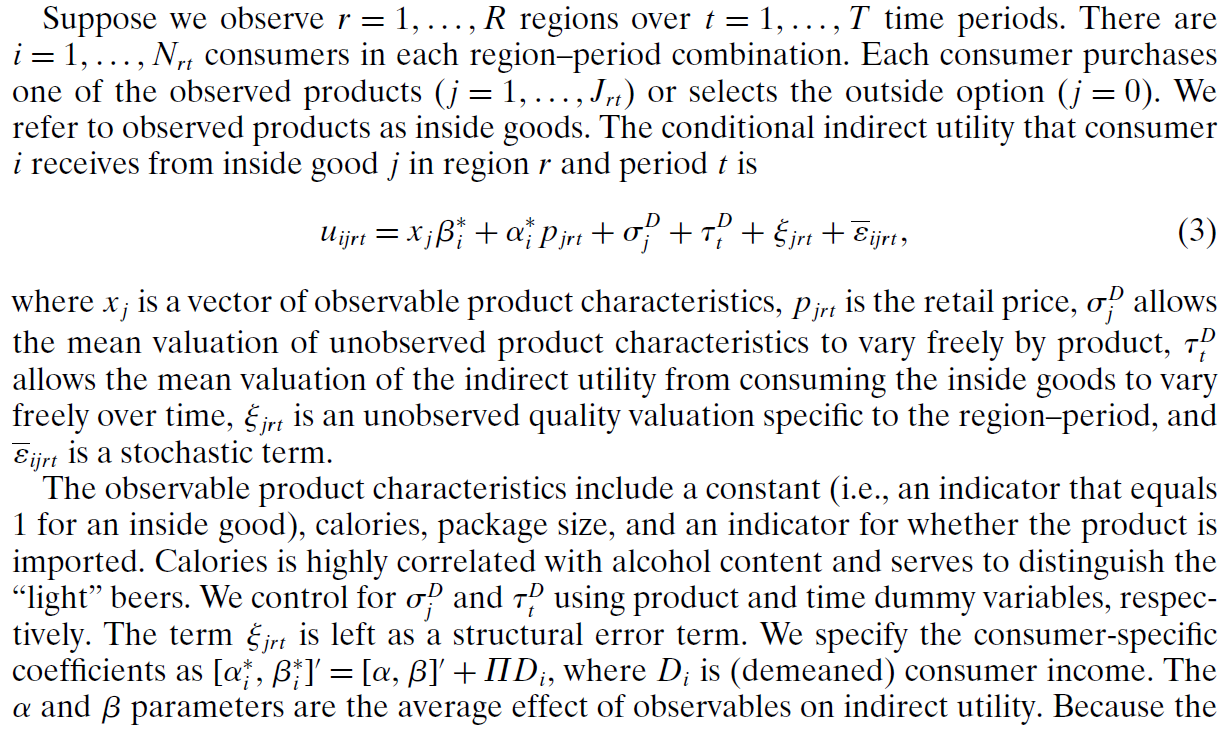
\includegraphics[width=0.95\linewidth]{eq_3}
    \end{center}    
\end{frame}

\begin{frame}\frametitle{Statistical Assumptions of Demand Model}
    \begin{center}
        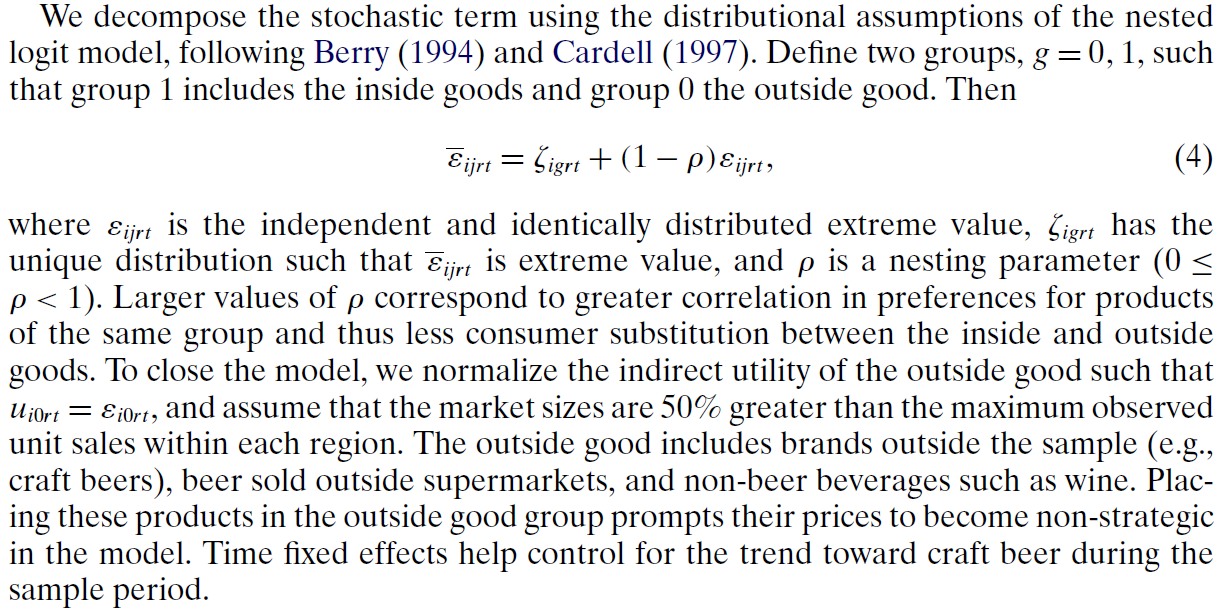
\includegraphics[width=0.95\linewidth]{eq_4}
    \end{center}
    This economic model of consumer demand probably does not make sense
    \begin{itemize}
        \item Do not worry, it will by the end of the semester!
    \end{itemize}
\end{frame}

\begin{frame}\frametitle{Implied Market Shares}
    This demand model implies that the market share for product $j$ in market $r$ in year $t$ is
    \begin{center}
        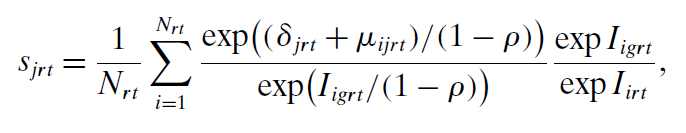
\includegraphics[width=0.6\linewidth]{eq_6}
    \end{center}
    where indirect utility has been rewritten as
    \begin{center}
        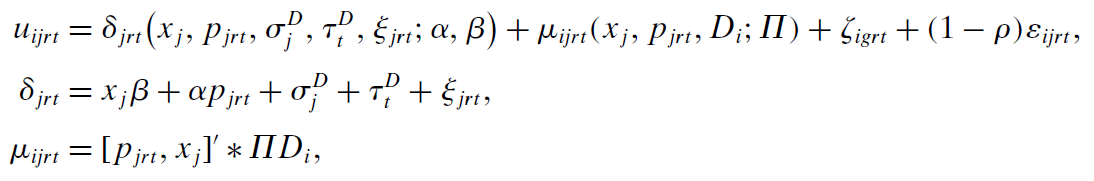
\includegraphics[width=0.9\linewidth]{eq_5}
    \end{center}
\end{frame}

\begin{frame}\frametitle{Estimation of Demand Model}
    If $\Pi = 0$, which means consumer preference do not vary with income, then the expression for market shares simplifies to
    \begin{center}
        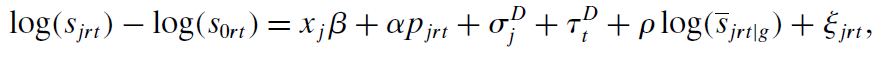
\includegraphics[width=0.8\linewidth]{eq_7}
    \end{center}
    which can be estimated with an OLS regression \\
    \vspace{2ex}
    To estimate the more general demand model without making this assumption, the authors 
    \begin{itemize}
        \item Derive moment conditions from this economic model
        \item Estimate its parameters using generalized method of moments (GMM)
    \end{itemize}
    \vspace{2ex}
    ``Moment conditions'' and ``GMM'' probably do not make sense
    \begin{itemize}
        \item Do not worry, they will by the end of the semester!
    \end{itemize}
\end{frame}

\begin{frame}\frametitle{Demand Estimation Results}
    These parameters define consumer preferences for product characteristics \\
    \begin{center}
        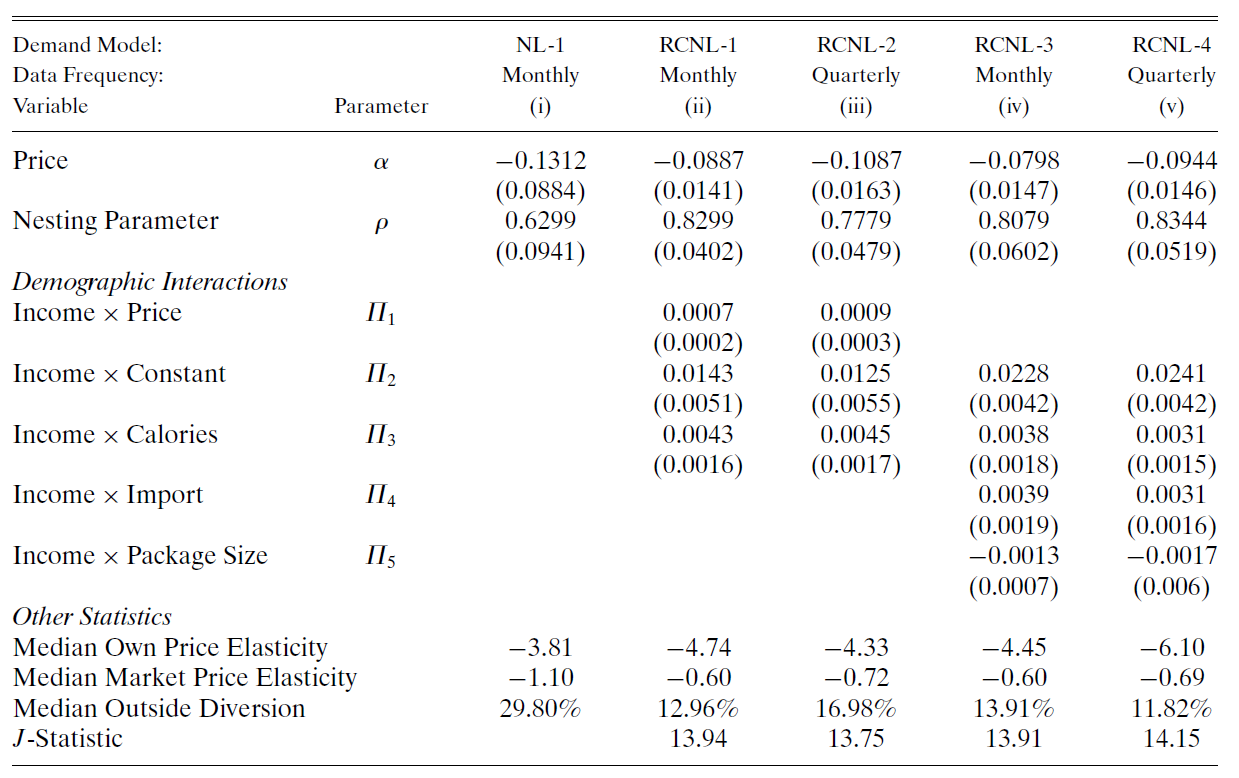
\includegraphics[width=0.9\linewidth]{table_4}
    \end{center}
\end{frame}

\begin{frame}\frametitle{Estimated Demand Elasticities}
    The authors combine these parameter estimates with their demand model to calculate own-price and cross-price elasticities
    \begin{center}
        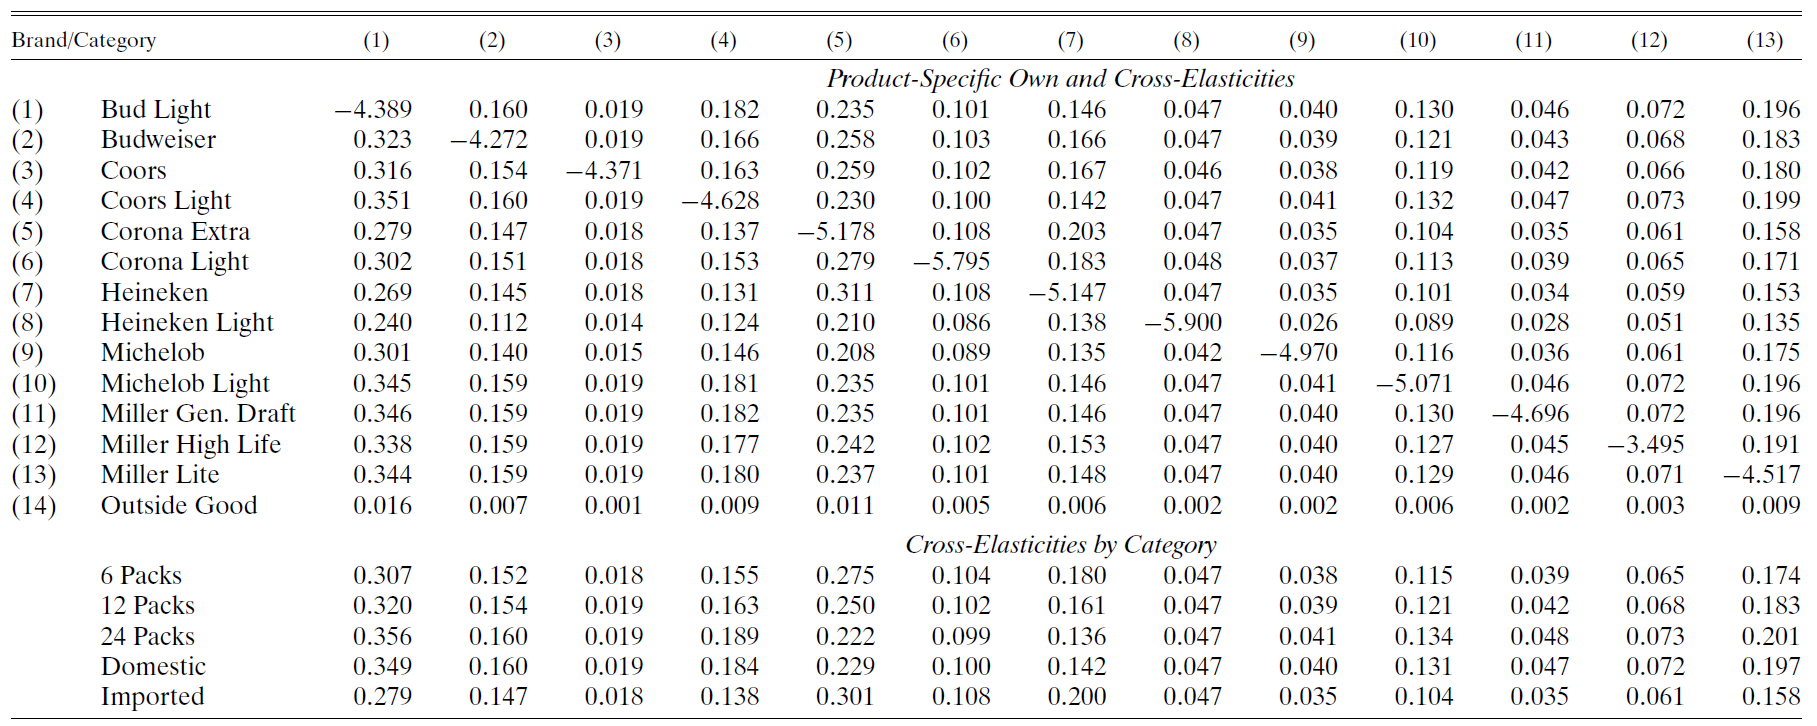
\includegraphics[width=0.95\linewidth]{table_5}
    \end{center}
    \begin{itemize}
        \item These elasticities would be difficult to generate from reduced-form regressions
    \end{itemize}
\end{frame}

\begin{frame}\frametitle{Economic Model of Supply (or Pricing)}
    The authors next model the supply side of the market \\
    \vspace{2ex}
    The resulting first-order condition gives equilibrium prices as a function of
    \begin{itemize}
        \item Marginal cost
        \item Market shares and elasticities
        \item Ownership structure
    \end{itemize}
    \begin{center}
        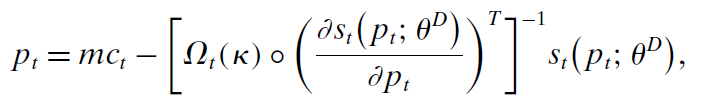
\includegraphics[width=0.6\linewidth]{eq_9}
    \end{center}
    where the ownership structure changes due to the merger
    \begin{center}
        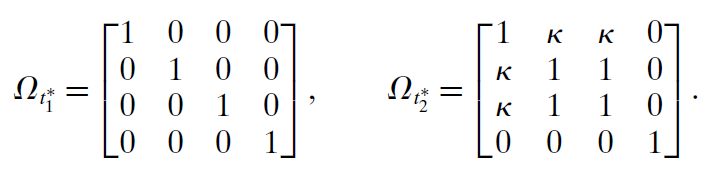
\includegraphics[width=0.6\linewidth]{eq_10}
    \end{center}
\end{frame}

\begin{frame}\frametitle{Statistical Assumptions of Supply Model}
    The authors do not observe marginal costs, so they model them as a function of transportation costs and unobservables
    \begin{center}
        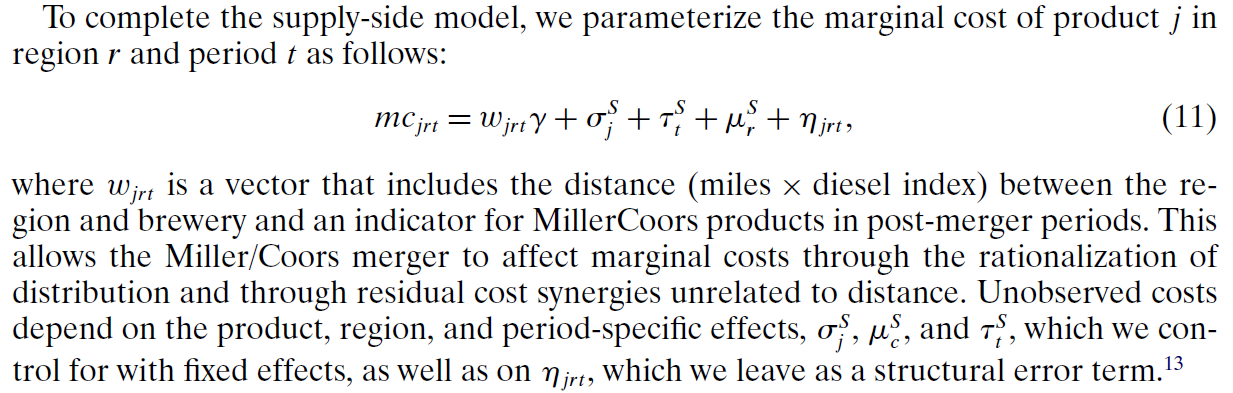
\includegraphics[width=0.95\linewidth]{eq_11}
    \end{center}
    They then construct supply-side moment conditions and estimate parameters using method of moments \\
    \vspace{2ex}
    Reminder: it is ok if this does not make sense right now!
    \begin{itemize}
        \item Just an example to show what structural estimation can achieve
    \end{itemize}
\end{frame}

\begin{frame}\frametitle{Supply Estimation Results}
    \begin{center}
        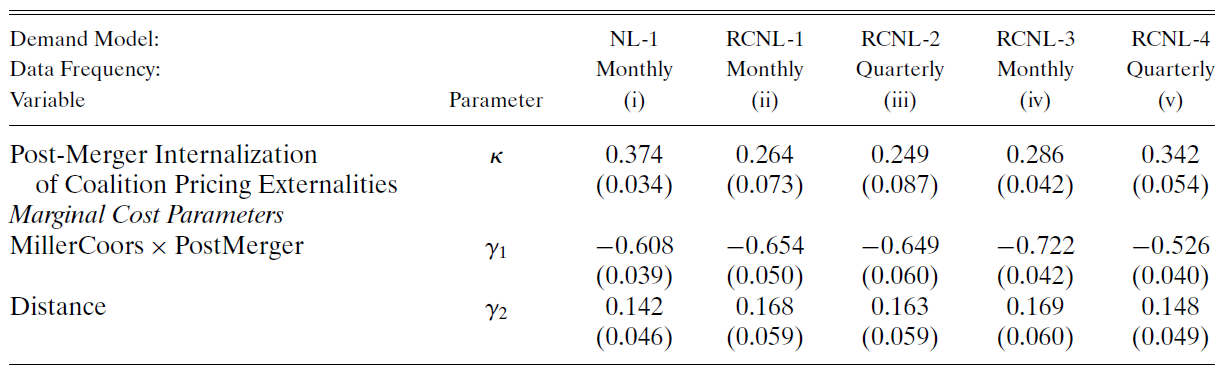
\includegraphics[width=0.95\linewidth]{table_6}
    \end{center}
    The parameter $\kappa$ captures the extent that one firm internalizes its price effects on the other firm's profits
    \begin{itemize}
        \item 25--34\% of these price effects are internalized
    \end{itemize}
    \vspace{2ex}
    The $\gamma$ parameters describe marginal costs
    \begin{itemize}
        \item Marginal cost of Coors Light fell by 14\% post-merger
        \item Transportation costs account for 2--3\% of retail prices
    \end{itemize}
\end{frame}

\begin{frame}\frametitle{Estimated Markups}
    The authors combine the estimated parameters with the economic model to calculate markups before and after the merger
    \begin{center}
        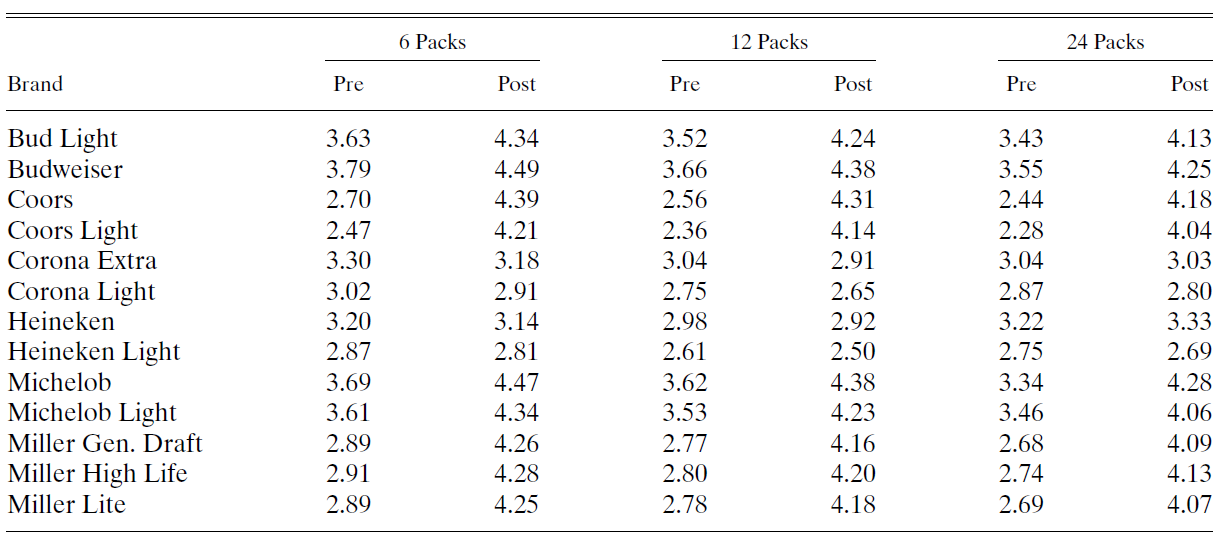
\includegraphics[width=0.95\linewidth]{table_7}
    \end{center}
    \begin{itemize}
        \item Markups increase substantially for MillerCoors and ABI beers, but not for import brands
    \end{itemize}    
\end{frame}

\begin{frame}\frametitle{Implied Cost Shocks}
    An alternate explanation for the observed prices is that ABI experiences a post-merger cost shock
    \begin{itemize}
        \item The authors estimate what cost shocks would have been required to explain the observed prices under each competitive regime
    \end{itemize}
    \begin{center}
        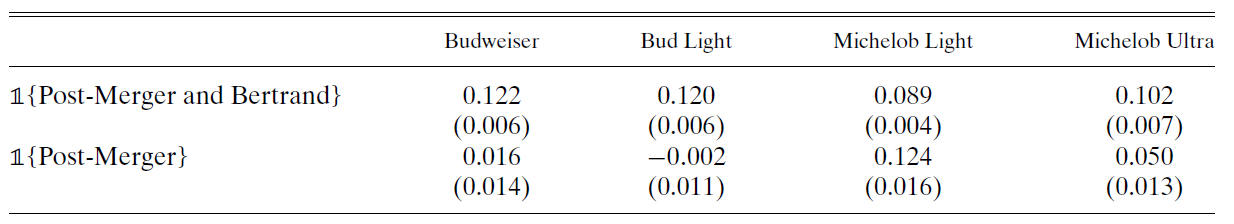
\includegraphics[width=0.95\linewidth]{table_8}
    \end{center}
    If firms priced unilaterally, ABI marginal cost increases of 12--21\% would be required to explain prices
    \
\end{frame}

\begin{frame}\frametitle{Counterfactual Price Simulations}
    The authors use their parameters and model to simulate price trajectories under a variety of counterfactual market assumptions
    \begin{center}
        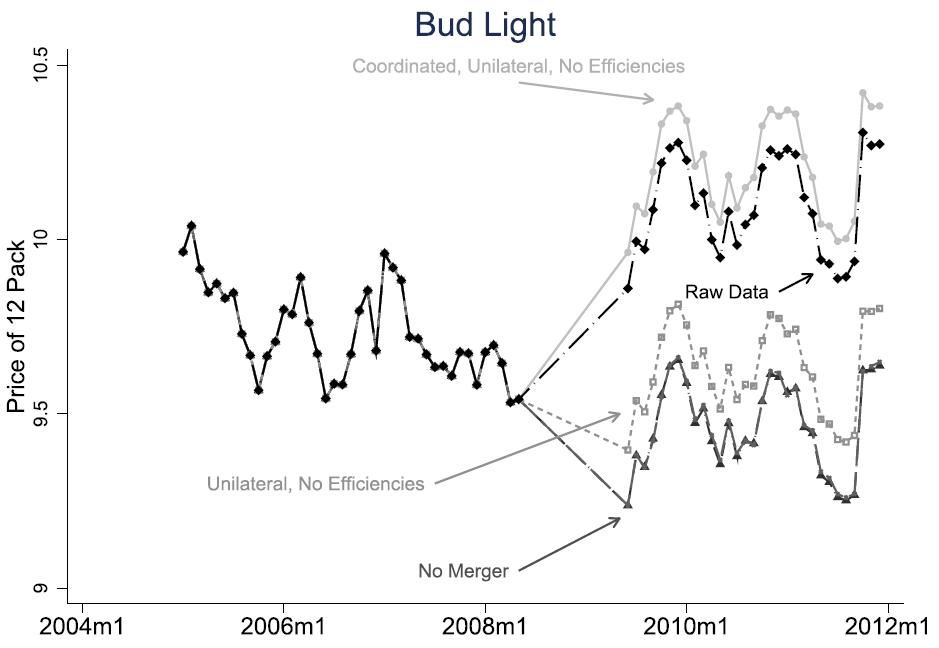
\includegraphics[width=0.7\linewidth]{fig_5}
    \end{center}
    \begin{itemize}
        \item ABI price increases are almost entirely due to coordinated pricing
    \end{itemize}
\end{frame}

\begin{frame}\frametitle{Welfare Calculations}
    The authors also calculate welfare effects for each counterfactual
    \begin{center}
        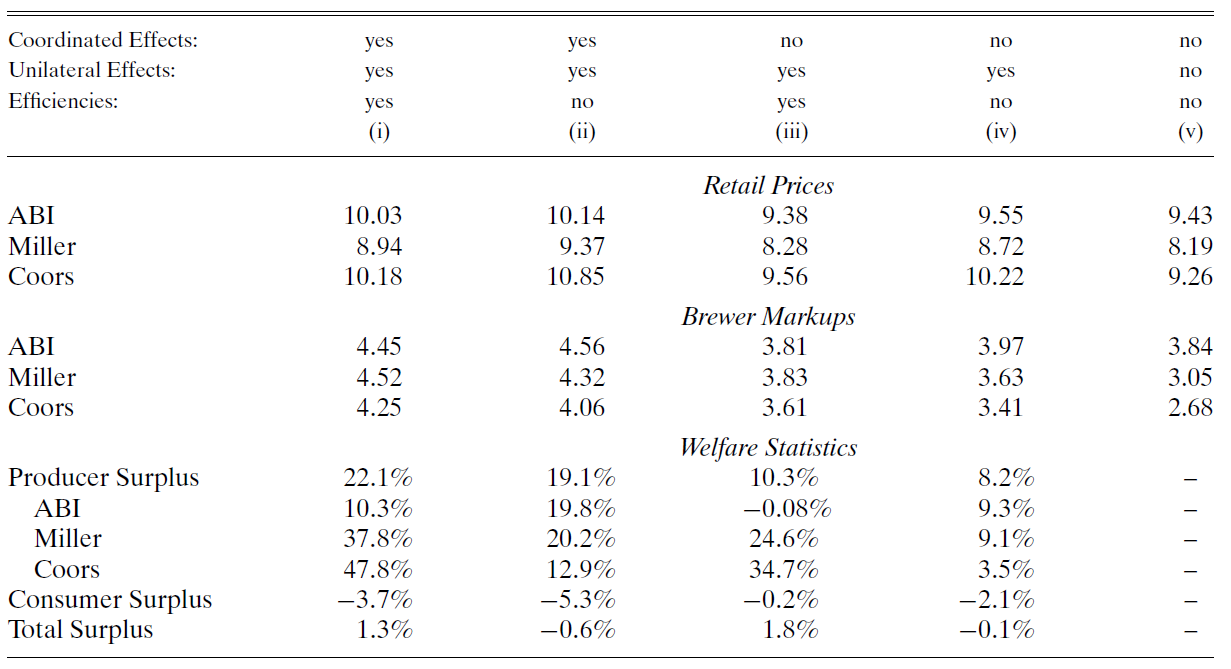
\includegraphics[width=0.85\linewidth]{table_10}
    \end{center}
    \begin{itemize}
        \item Welfare effects depend on whether cost efficiencies are realized and whether pricing is coordinated
        \item Merger could improve total surplus under reasonable assumptions
    \end{itemize}
\end{frame}

\end{document}